\chapter{Complex Numbers}

\paragraph{Prerequisites.} \nameref{sec:Polar-Coordinates}
\paragraph{Exercises.} \nameref{sec:A10.1}, \nameref{sec:A10.2}, \nameref{sec:A10.3}, \nameref{sec:A10.4}

\section{Complex Numbers in Cartesian Form}

\begin{definition}
    The \vocab{imaginary unit} $\i$ is a root to the equation \[x^2 + 1 = 0.\]
\end{definition}

\begin{definition}
    A \vocab{complex number} $z$ has \vocab{Cartesian form} $x + \i y$, where $x$ and $y$ are real numbers. We call $x$ the \vocab{real part} of $z$, denoted $\Re z$. Likewise, we call $y$ the \vocab{imaginary part} of $z$, denoted $\Im z$.
\end{definition}

\begin{definition}
    The set of complex numbers is denoted $\CC$ and is defined as \[\CC = \bc{z : z = x + \i y , \quad x, y \in \RR}.\]
\end{definition}
\begin{remark}
    The set of real numbers, $\RR$, is a proper subset of the set of complex numbers, $\CC$. That is, $\RR \subset \CC$.
\end{remark}

\begin{proposition}
    Complex numbers cannot be ordered.
\end{proposition}
\begin{proof}
    Seeking a contradiction, suppose $\i > 0$. Multiplying both sides by $\i$, we have $\i^2 = -1 > 0$, a contradiction. Hence, we must have $\i < 0$. However, multiplying both sides by $\i$ and changing signs (since $\i < 0$), we have $\i^2 = -1 > 0$, another contradiction. Thus, $\CC$ cannot be ordered.
\end{proof}

\begin{definition}
    Let $z = x + \i y$. $z$ is said to be \vocab{purely real} if and only if $y = 0$. Likewise, $z$ is said to be \vocab{purely imaginary} if and only if $x = 0$.
\end{definition}

\subsection{Complex Numbers in Cartesian Form}

\begin{definition}
    The \vocab{modulus} of a complex number $z$ is denoted $\abs{z}$ and is defined as \[\abs{z} = \sqrt{\Re{z}^2 + \Im{z}^2}.\]
\end{definition}

\begin{fact}[Algebraic Operations on Complex Numbers]
    Let $z_1, z_2, z_3 \in \CC$.
    \begin{itemize}
        \item Two complex numbers are equal if and only if their corresponding real and imaginary parts are equal. \[z_1 = z_2 \iff \Re z_1 = \Re z_2 \land \Im z_1 = \Im z_2.\]
        \item Addition of complex numbers is commutative, i.e. \[z_1 + z_2 = z_2 + z_1\] and associative, i.e. \[(z_1 + z_2) + z_3 = z_1 + (z_2 + z_3).\]
        \item Multiplication of complex numbers is commutative, i.e. \[z_1z_2 = z_2z_1,\] associative, i.e. \[z_1(z_2z_3) = (z_1z_2)z_3\] and distributive, i.e. \[z_1(z_2 + z_3) = z_1z_2 + z_1z_3.\]
    \end{itemize}
\end{fact}

\begin{definition}
    The \vocab{conjugate} of the complex number $z = x + \i y$ is denoted $z\conj$ with definition \[z\conj = x - \i y.\] We refer to $z$ and $z\conj$ as a \vocab{conjugate pair} of complex numbers.
\end{definition}

\begin{fact}[Properties of Complex Conjugates]
    \phantom{.}
    \begin{itemize}
        \item (distributive over addition) $(z + w)\conj = z\conj + w\conj$.
        \item (distributive over multiplication) $(zw)\conj = z\conj w\conj$.
        \item (involution) $\bp{z\conj}\conj = z$.
        \item $z + z\conj = 2\Re{z}$.
        \item $z - z\conj = 2\Im{z} \i$.
        \item $z z\conj = \Re{z}^2 + \Im{z}^2 = \abs{z}^2$.
    \end{itemize}
\end{fact}
\begin{remark}
    Because conjugation is distributive over addition and multiplication, we also have the following identities: \[(kz)\conj = k z\conj, \qquad \bp{z^n}\conj = \bp{z\conj}^n,\] where $k \in \RR$ and $n \in \ZZ$.
\end{remark}

\begin{proposition}[Division of Complex Numbers]
    For all non-zero complex numbers, \[z^{-1} = \frac{z\conj}{\abs{z}^2}.\]
\end{proposition}
\begin{proof}
    Multiplying by $\frac{z\conj}{z\conj}$, we have \[\frac{1}{z} = \frac{z\conj}{z z\conj} = \frac{z\conj}{\abs{z}^2}.\]
\end{proof}

\subsection{Roots of Polynomial Equations}

\begin{theorem}[Fundamental Theorem of Algebra]
    A non-zero, single-variable, degree $n$ polynomial with complex coefficients has $n$ roots in $\CC$, counted with multiplicity.
\end{theorem}

\begin{theorem}[Conjugate Root Theorem]
    For a polynomial equation with all real coefficients, non-real roots must occur in conjugate pairs.
\end{theorem}
\begin{proof}
    Suppose $z$ is a non-real root to the polynomial $P(z) = a_n z^n + a_{n-1} z^{n-1} + \dots + a_1 z + a_0$, where $a_n, a_{n-1}, \dots, a_1, a_0 \in \RR$. Consider $P(z\conj)$. \[P(z\conj) = a_n \bp{z\conj}^n + a_{n-1} \bp{z\conj}^{n-1} + \dots + a_1 \bp{z\conj} + a_0.\] By conjugation properties, this simplifies to \[P(z\conj) = \bp{a_n z^n + a_{n-1} z^{n-1} + \dots + a_1 z + a_0}\conj,\] which clearly evaluates to 0, whence $z\conj$ is also a root of $P(z)$.
\end{proof}

\section{Complex Numbers in Polar Form}

\subsection{Geometrical Representation of a Complex Number}

\begin{definition}
    The \vocab{Argand diagram} is a modified Cartesian plane where the $x$-axis represents real numbers and the $y$-axis represents imaginary numbers. The two axes are called the \vocab{real axis} and \vocab{imaginary axis} correspondingly.

    On the Argand diagram, the complex number $z = x + \i y$, where $x, y \in \RR$, can be represented by
    \begin{itemize}
        \item the point $Z(x, y)$ or $Z(z)$; or
        \item the vector $\oa{OZ}$.
    \end{itemize}

    \begin{center}\tikzsetnextfilename{339}
        \begin{tikzpicture}[scale=0.8, trim axis left, trim axis right]
            \begin{axis}[
                domain = 0:10,
                samples = 101,
                axis y line=middle,
                axis x line=middle,
                xtick = \empty,
                ytick = \empty,
                xmax=8,
                xmin=-2,
                ymin=-2,
                ymax=8,
                xlabel = {$\Re$},
                ylabel = {$\Im$},
                legend cell align={left},
                legend pos=outer north east,
                after end axis/.code={
                    \path (axis cs:0,0) 
                        node [anchor=north east] {$O$};
                    }
                ]
    
                \coordinate[label=above:$Z\bp{x, y} \lor Z\bp{z}$] (Z) at (5, 6);
                \coordinate (O) at (0, 0);
    
                \draw[->-=0.5, very thick] (O) -- (Z);
                \node[anchor=north west] at (2.5, 3) {$\oa{OZ}$};
    
                \fill (Z) circle[radius=2.5pt];
            \end{axis}
        \end{tikzpicture}
    \end{center}
\end{definition}

In an Argand diagram, let the points $Z$ and $W$ represent the complex numbers $z$ and $w$ respectively. Then $\oa{OZ}$ and $\oa{OW}$ are the corresponding vectors representing $z$ and $w$.

The following diagram shows the geometrical effect of addition on complex numbers. Here, the point $P$ represents the complex number $z + w$. Observe that $OWPZ$ is a parallelogram (due to the parallelogram law of vector addition).

\begin{center}\tikzsetnextfilename{340}
    \begin{tikzpicture}[trim axis left, trim axis right]
        \begin{axis}[
            domain = 0:10,
            samples = 101,
            axis y line=middle,
            axis x line=middle,
            xtick = \empty,
            ytick = \empty,
            xmax=8,
            xmin=-2,
            ymin=-2,
            ymax=8,
            xlabel = {$\Re$},
            ylabel = {$\Im$},
            legend cell align={left},
            legend pos=outer north east,
            after end axis/.code={
                \path (axis cs:0,0) 
                    node [anchor=north east] {$O$};
                }
            ]

            \coordinate[label=right:$Z\bp{z}$] (Z) at (4, 1);
            \coordinate[label=above:$W\bp{w}$] (W) at (2, 3);
            \coordinate[label=above:$P\bp{z + w}$] (P) at (6, 4);
            \coordinate (O) at (0, 0);

            \draw[->-=0.5, very thick] (O) -- (Z);
            \draw[->-=0.5, very thick] (O) -- (W);
            \draw[->-=0.5, very thick] (O) -- (P);
            \draw[dotted, ->-=0.5] (Z) -- (P);
            \draw[dotted, ->-=0.5] (W) -- (P);
        \end{axis}
    \end{tikzpicture}
\end{center}

The following diagram shows the geometrical effect of multiplying a complex number by a real number $k$. Here, $Z_1$ represents a point where $k > 1$, $Z_2$ where $0 < k < 1$, and $Z_3$ where $k < 0$. Observe that the points lie on the straight line passing through the origin $O$ and the point $Z$.

\begin{center}\tikzsetnextfilename{341}
    \begin{tikzpicture}[trim axis left, trim axis right]
        \begin{axis}[
            domain = 0:10,
            samples = 101,
            axis y line=middle,
            axis x line=middle,
            xtick = \empty,
            ytick = \empty,
            xmax=5,
            xmin=-5,
            ymin=-5,
            ymax=5,
            xlabel = {$\Re$},
            ylabel = {$\Im$},
            legend cell align={left},
            legend pos=outer north east,
            after end axis/.code={
                \path (axis cs:0,0) 
                    node [anchor=north east] {$O$};
                }
            ]

            \coordinate[label=above:$Z$] (Z) at (2, 1);
            \coordinate (O) at (0, 0);

            \draw (-5, -2.5) -- (5, 2.5);
            \draw[very thick] (O) -- (Z);

            \fill (Z) circle[radius=2.5pt];
            \fill (-2.5, -1.25) circle[radius=2.5pt];
            \fill (3, 1.5) circle[radius=2.5pt];
            \fill (1, 0.5) circle[radius=2.5pt];

            \node[anchor=north] at (-2.5, -1.25) {$Z_3$};
            \node[anchor=south] at (1, 0.5) {$Z_2$};
            \node[anchor=south] at (3, 1.5) {$Z_1$};
        \end{axis}
    \end{tikzpicture}
\end{center}

\begin{definition}
    The \vocab{argument} of a complex number $z$ is the directed angle $\t$ that $Z(z)$ makes with the positive real axis, and is denoted by $\arg{z}$. Note that $\arg{z} > 0$ when measured in an anticlockwise direction from the positive real axis, and $\arg{z} < 0$ when measured in a clockwise directoin from the positive real axis.
\end{definition}

Note that $\arg{z}$ is not unique; the position of $Z(z)$ is not affected by adding an integer multiple of $2\pi$ to $\t$. Therefore, if $\arg{z} = \f$, then $\f + 2k\pi$, where $k \in \ZZ$, is also an argument of $z$. We hence introduce the principal argument of $z$.

\begin{definition}
    The value of $\arg{z}$ in the interval $(-\pi, \pi]$ is known as the \vocab{principal argument} of $z$.
\end{definition}

The modulus $r = \abs{z}$ and argument $\t = \arg{z}$ of a complex number $z$ can easily be identified on an Argand diagram:

\begin{center}\tikzsetnextfilename{342}
    \begin{tikzpicture}[scale=0.8, trim axis left, trim axis right]
        \begin{axis}[
            domain = 0:10,
            samples = 101,
            axis y line=middle,
            axis x line=middle,
            xtick = \empty,
            ytick = \empty,
            xmin=-2,
            xmax=8,
            ymin=-2,
            ymax=8,
            xlabel = {$\Re$},
            ylabel = {$\Im$},
            legend cell align={left},
            legend pos=outer north east,
            after end axis/.code={
                \path (axis cs:0,0) 
                    node [anchor=north east] {$O$};
                }
            ]

            \coordinate (A) at (4, 0);
            \coordinate (B) at (0, 0);
            \coordinate (C) at (3, 4);

            \fill (3, 4) circle[radius=2.5pt];
            \draw (0, 0) -- (3, 4);
            \node[anchor=south east] at (1.5, 2) {$r$};
            \node[anchor=south] at (3, 4) {$Z(z)$};

            \draw pic [draw, angle radius=10mm, "$\t$"] {angle = A--B--C};
        \end{axis}
    \end{tikzpicture}
\end{center}

\subsection{Complex Numbers in Polar Form}

\begin{definition}
    The \vocab{trigonometric form} of the complex number $z$ is \[z = r\bp{\cos \t + \i \sin \t},\] where $r = \abs{z}$ and $\t = \arg{z}$, $-\pi < \t \leq \pi$.
\end{definition}
\begin{sketch}
    Let $z = x + \i y$, where $x, y \in \RR$. From the diagram above, we see that $x = r\cos\t$ and $y = r\sin\t$. Hence, \[z = x + \i y = (r\cos\t) + \i (r\sin\t) = r \bp{\cos \t + \i \sin\t}.\]
\end{sketch}

\begin{theorem}[Euler's Identity]
    For all $\t \in \RR$, \[\e^{\i \t} = \cos \t + \i \sin \t.\]
\end{theorem}
\begin{proof}[Proof 1 (Series Expansion)]
    By the standard series expansion of $\e^x$, we have \[\e^{\i \t} = 1 + \i \t + \frac{(\i \t)^2}{2!} + \frac{(\i \t)^3}{3!} + \frac{(\i \t)^4}{4!} + \frac{(\i \t)^5}{5!} + \dots.\] Simplifying and grouping real and imaginary parts together, \[\e^{\i \t} = \bp{1 - \frac{\t^2}{2!} + \frac{\t^4}{4!} + \dots} + \i \bp{\t - \frac{\t^3}{3!} + \frac{\t^5}{5!} + \dots},\] which we recognize to be the standard series expansions of $\cos \t$ and $\sin \t$ respectively. Hence, \[\e^{\i \t} = \cos \t + \i \sin \t.\]
\end{proof}
\begin{proof}[Proof 2 (Differentiation)]
    Let $f(\t) = \e^{-\i \t} \bp{\cos \t + \i \sin \t}$. Differentiating with respect to $\t$, \[f'(\t) = \e^{-\i \t} \bp{-\sin \t + \i \cos \t} - \i \e^{-\i \t} \bp{\cos \t + \i \sin \t} = 0.\] Hence, $f(\t)$ is constant. Evaluating $f(\t)$ at $\t = 0$, we have $f(\t) = 1$, whence \[\e^{-\i \t} \bp{\cos \t + \i \sin \t} = 1 \implies \e^{\i \t} = \cos \t + \i \sin \t.\]
\end{proof}

\begin{definition}
    The \vocab{exponential form} of the complex number $z$ is \[z = r \e^{\i \t},\] where $r = \abs{z}$ and $\t = \arg{z}$, $-\pi < \t \leq \pi$.
\end{definition}

Both the trigonometric and exponential forms of writing a complex number $z$ are collectively known as the \vocab{polar form} of $z$.

We now observe the geometrical effect of complex conjugation on an Argand diagram. Let $Z$ be the point representing $z = x + \i y$ and $P$ be the point representing $z\conj = x - \i y$. Then $P$ is the reflection of $Z$ in the real axis, as shown below:

\begin{center}\tikzsetnextfilename{343}
    \begin{tikzpicture}[scale=0.8, trim axis left, trim axis right]
        \begin{axis}[
            domain = 0:10,
            samples = 101,
            axis y line=middle,
            axis x line=middle,
            xtick = \empty,
            ytick = \empty,
            xmin=-2,
            xmax=8,
            ymin=-5,
            ymax=5,
            xlabel = {$\Re$},
            ylabel = {$\Im$},
            legend cell align={left},
            legend pos=outer north east,
            after end axis/.code={
                \path (axis cs:0,0) 
                    node [anchor=north east] {$O$};
                }
            ]

            \coordinate (B) at (0, 0);
            \coordinate (Z) at (5, 3);
            \coordinate (P) at (5, -3);
            \coordinate (E) at (5, 0);

            \fill (Z) circle[radius=2.5pt];
            \fill (P) circle[radius=2.5pt];
            \draw (B) -- (Z);
            \draw (B) -- (P);
            \node[anchor=south] at (Z) {$Z(z)$};
            \node[anchor=north] at (P) {$P(z\conj)$};
            \draw[dotted] (Z) -- (P);

            \draw (4.8, 1.5) -- (5.2, 1.5);
            \draw (4.8, -1.5) -- (5.2, -1.5);

            \draw pic [draw, angle radius=3mm] {right angle = Z--E--B};
            \draw pic [draw, angle radius=3mm] {right angle = P--E--B};
        \end{axis}
    \end{tikzpicture}
\end{center}

From the diagram, it is obvious that

\begin{proposition}[Conjugation in Polar Form]
    If $z = r \e^{\i \t}$, then $z\conj = r\e^{\i \t}$. Also, \[\arg{z\conj} = -\t = -\arg{z}, \qquad \abs{z} = r = \abs{z \conj}.\]
\end{proposition}

Recall that $z + z\conj = 2\Re{z}$ and $z - z\conj = 2 \Im{z} \i$. Using the proposition above, we have a similar result when $z$ is written in polar form:

\begin{proposition}
    \[\e^{\i \t} + \e^{-\i \t} = 2\cos \t, \qquad \e^{\i \t} - \e^{-\i \t} = \bp{2 \sin \t} \i.\]
\end{proposition}
\begin{proof}
    Convert $\e^{\i \t}$ and $\e^{-\i \t}$ into trigonometric form and simplify.
\end{proof}

Lastly, we observe the effect of multiplication and division on the modulus and argument of complex numbers.

\begin{proposition}[Multiplication in Polar Form]
    Let $z_1 = r_1 \e^{\i \t_1}$ and $z_2 = r_2 \e^{\i \t_2}$. Then \[\abs{z_1 z_2} = r_1 r_2 = \abs{z_1} \abs{z_2}, \qquad \arg{z_1 z_2} = \t_1 + \t_2 = \arg{z_1} + \arg{z_2}.\]
\end{proposition}
\begin{proof}
    Observe that \[z_1 z_2 = \bp{r_1 \e^{\i \t_1}}\bp{r_2 \e^{\i \t_2}} = (r_1 r_2) \e^{\i (\t_1 + \t_2)}.\] The results follow immediately.
\end{proof}

\begin{corollary}[Exponentiation in Polar Form]
    For $n \in \ZZ$, \[\abs{z^n} = r^n = \abs{z}^n, \qquad \arg{z^n} = n \t = n \arg{z}.\]
\end{corollary}
\begin{proof}
    Repeatedly apply the above proposition.
\end{proof}

\begin{proposition}[Division in Polar Form]
    Let $z_1 = r_1 \e^{\i \t_1}$ and $z_2 = r_2 \e^{\i \t_2}$. Then \[\abs{\frac{z_1}{z_2}} = \frac{r_1}{r_2} = \frac{\abs{z_1}}{\abs{z_2}}, \qquad \arg{\frac{z_1}{z_2}} = \t_1 - \t_2 = \arg{z_1} - \arg{z_2}.\]
\end{proposition}
\begin{proof}
    Observe that \[\frac{z_1}{z_2} = \frac{r_1 \e^{\i \t_1}}{r_2 \e^{\i \t_2}} = \frac{r_1}{r_2} \e^{\i (\t_1 - \t_2)}.\] The results follow immediately.
\end{proof}

\section{Geometrical Effects and De Moivre's Theorem}

\subsection{Geometrical Effect of Multiplying Complex Numbers}

Let points $P$, $Q$ and $R$ represent the complex numbers $z_1$, $z_2$ and $z_3$ respectively, as illustrated in the Argand diagram below.

\begin{center}\tikzsetnextfilename{344}
    \begin{tikzpicture}[trim axis left, trim axis right]
        \begin{axis}[
            domain = 0:10,
            samples = 101,
            axis y line=middle,
            axis x line=middle,
            xtick = \empty,
            ytick = \empty,
            xmax=3,
            xmin=-6,
            ymin=-2,
            ymax=7,
            xlabel = {$\Re$},
            ylabel = {$\Im$},
            legend cell align={left},
            legend pos=outer north east,
            after end axis/.code={
                \path (axis cs:0,0) 
                    node [anchor=north east] {$O$};
                }
            ]

            \coordinate (O) at (0, 0);
            \coordinate[label=above:$P(z_1)$] (P) at (-1, 3);
            \coordinate[label=above:$Q(z_2)$] (Q) at (2, 1);
            \coordinate[label=above:$R(z_1 z_2)$] (R) at (-5, 5);
            \coordinate (M) at (5, 0);
            \coordinate (N) at (-5, 0);

            \fill (P) circle[radius=2.5pt];
            \fill (Q) circle[radius=2.5pt];
            \fill (R) circle[radius=2.5pt];

            \draw[very thick] (O) -- (R);
            \draw[dotted] (O) -- (P);
            \draw[dotted] (O) -- (Q);

            \node[anchor=west] at ($(O)!0.7!(P)$) {$r_1$};
            \node[anchor=north west] at ($(O)!0.7!(Q)$) {$r_2$};
            \node[anchor=south west] at ($(O)!0.7!(R)$) {$r_1 r_2$};


            \draw pic [draw, angle radius=8mm] {angle = M--O--P};
            \draw pic [draw, angle radius=6mm] {angle = M--O--Q};
            \draw pic [draw, angle radius=6mm] {angle = P--O--R};

            \node[anchor=north] at (0.6, 0) {$\t_2$};
            \node at (-0.8, 1.4) {$\t_2$};
            \node at (0.3, 0.8) {$\t_1$};
        \end{axis}
    \end{tikzpicture}
\end{center}

Geometrically, the point $R(z_1 z_2)$ is obtained by
\begin{enumerate}
    \item scaling by a factor of $r_2$ on $\oa{OP}$ to obtain a new modulus of $r_1 r_2$, followed by
    \item rotating $\oa{OP}$ through an angle $\t_2$ about $O$ in an anti-clockwise direction if $\t_2 > 0$ to obtain a new argument $\t_1 + \t_2$ (or in a clockwise direction if $\t_2 < 0$).
\end{enumerate}

\subsection{De Moivre's Theorem and its Applications}

\begin{theorem}[De Moivre's Theorem]
    For $n \in \QQ$, if $z = r\bp{\cos \t + \i \sin \t} = r \e^{\i \t}$, then \[z^n = r^n \bp{\cos n\t + \i \sin n\t} = r^n \e^{\i n \t}.\]
\end{theorem}
\begin{proof}
    Write $z^n$ in exponential form before converting it into trigonometric form.
\end{proof}

We now discuss some of the applications of De Moivre's theorem.

\begin{method}[Finding $n$th Roots]
    Suppose we want to find the $n$th roots of a complex number $w = r \e^{\i \t}$. We begin by setting up the equation \[z^n = w = r \e^{\i \bp{\t + 2k\pi}},\] where $k \in \ZZ$. Next, we take $n$th roots on both sides, which yields \[z = r^{1/n} \e^{\i \bp{\t + 2k\pi} /n}.\] Lastly, we pick values of $k$ such that $\arg z = \frac{\t + 2k\pi}{n}$ lies in the principal interval $(-\pi, \pi]$.
\end{method}

\begin{definition}
    Let $n \in \ZZ$. The \vocab{$n$th roots of unity} are the $n$ solutions to the equation \[z^n - 1 = 0.\]
\end{definition}

\begin{proposition}[Roots of Unity in Polar Form]
    The $n$th roots of unity are given by \[z = \cos \frac{2k \pi}{n} + \i \sin \frac{2k \pi}{n} = \e^{\i \bp{2k \pi / n}},\] where $k \in \ZZ$.
\end{proposition}
\begin{proof}
    Use De Moivre's theorem.
\end{proof}

\begin{fact}{Geometric Properties of Roots of Unity}
    On an Argand diagram, the $n$th roots of unity
    \begin{itemize}
        \item all lie on a circle of radius 1.
        \item are equally spaced apart.
        \item form a regular $n$-gon.
    \end{itemize}
\end{fact}

De Moivre's theorem can also be used to derive trigonometric identities. The trigonometric identities you will be required to prove typically involve reducing ``powers'' to ``multiple angles'' (e.g. expressing $\sin^3 \t$ in terms of $\sin \t$ and $\sin 3\t$), or vice versa (e.g. expressing $\sin 3\t$ in terms of $\sin \t$ and $\sin^3 \t$).

\begin{proposition}[Power to Multiple Angles]
    Let $z = \cos \t + \i \sin \t = \e^{\i \t}$. Then \[z^n + z^{-n} = 2\cos n\t, \qquad z^n - z^{-n} = 2\i \sin n\t.\]
\end{proposition}

\begin{method}[Multiple Angles to Powers]
    Suppose we want to express $\cos n\t$ and $\sin n\t$ in terms of powers of $\sin \t$ and $\cos \t$. We begin by invoking De Moivre's theorem: \[\cos n\t + \i \sin n\t = \bp{\cos \t + \i \sin \t}^n.\] Next, using the binomial theorem, \[\cos n\t + \i \sin n\t = \sum_{k = 0}^n \binom{n}{k} \cos^k \t \sin^{n-k} \t.\] We then take the real and imaginary parts of both sides to isolate $\cos n\t$ and $\sin n\t$: \[\cos n\t = \Re \sum_{k = 0}^n \binom{n}{k} \cos^k \t \sin^{n-k} \t, \qquad \sin n\t = \Im \sum_{k = 0}^n \binom{n}{k} \cos^k \t \sin^{n-k} \t.\]
\end{method}

\begin{example}
    Suppose we want to write $\sin 2\t$ in terms of $\sin \t$ and $\cos \t$. Using De Moivre's theorem, \[\cos 2\t + \i \sin 2\t = \bp{\cos \t + \i \sin \t}^2 = \cos^2 \t + 2\i \cos \t \sin \t - \sin^2 \t.\] Comparing imaginary parts, we obtain \[\sin 2\t = 2\cos\t\sin\t\] as expected.
\end{example}

Another way to derive new trigonometric identities is to differentiate known identities.

\begin{example}
    Using the ``power to multiple angle'' formula above, one can show that \[\cos^6 \t = \frac1{32} \bp{\cos 6\t + 6\cos4\t + 15\cos2\t + 10}.\] Differentiating, we obtain a new trigonometric identity: \[\sin \t \cos^5 \t = \frac1{32} \bp{\sin 6\t + 4\sin 4\t + 5\sin 2\t}.\]
\end{example}

\section{Loci in Argand Diagram}

\begin{definition}
    The \vocab{locus} (plural: loci) of a variable point is the path traced out by the point under certain conditions.
\end{definition}

\subsection{Standard Loci}

\begin{fact}[Circle]
    For $\abs{z-a} = r$, with $P$ representing the complex number $z$ and $A$ representing the fixed complex number $a$ and $r > 0$, the locus of $P$ is a circle with centre $A$ and radius $r$.

    \begin{center}\tikzsetnextfilename{345}
        \begin{tikzpicture}[trim axis left, trim axis right]
            \begin{axis}[
                domain = 0:10,
                samples = 101,
                axis y line=middle,
                axis x line=middle,
                xtick = \empty,
                ytick = \empty,
                xmax=11.5,
                xmin=-5.5,
                ymin=-4,
                ymax=11,
                xlabel = {$\Re$},
                ylabel = {$\Im$},
                legend cell align={left},
                legend pos=outer north east,
                legend style={fill=none},
                after end axis/.code={
                    \path (axis cs:0,0) 
                        node [anchor=north east] {$O$};
                    }
                ]
    
                \coordinate (O) at (0, 0);
                \coordinate[label=above:$A$] (C) at (3, 4);

                \fill (C) circle[radius=2.5pt];

                \draw[<->] (O) -- (C);

                \node[anchor=west] at (1.7, 2) {$r$};

                \draw[plotRed] (C) circle[radius=5];
                
                \addlegendimage{no markers, plotRed}
                \addlegendentry{locus of $P$};
            \end{axis}
        \end{tikzpicture}
    \end{center}
\end{fact}

\begin{fact}[Perpendicular Bisector]
    For $\abs{z - a} = \abs{z - b}$, with $P$ representing the complex number $z$, points $A$ and $B$ representing the fixed complex numbers $a$ and $b$ respectively, the locus of $P$ is the perpendicular bisector of the line segment joining $A$ and $B$.

    \begin{center}\tikzsetnextfilename{346}
        \begin{tikzpicture}[trim axis left, trim axis right]
            \begin{axis}[
                domain = -10:10,
                samples = 101,
                axis y line=middle,
                axis x line=middle,
                xtick = {-2},
                ytick = {1},
                yticklabels = {},
                xticklabels = {$B$},
                xmax=2,
                xmin=-3,
                ymin=-2,
                ymax=2,
                xlabel = {$\Re$},
                ylabel = {$\Im$},
                legend cell align={left},
                legend pos=outer north east,
                legend style={fill=none},
                after end axis/.code={
                    \path (axis cs:0,0) 
                        node [anchor=north west] {$O$};
                    }
                ]
    
                \coordinate (Z1) at (-2, 0);
                \coordinate (Z2) at (0, 1);
                \coordinate (O) at (0, 0);

                \draw[dotted] (Z1) -- (Z2);

                \addplot[plotRed] {-2*x - 1.5};
        
                \fill (Z1) circle[radius=2.5pt];
                \fill (Z2) circle[radius=2.5pt];

                \addlegendentry{locus of $P$};

                \coordinate (Z3) at (0, -1.5);
                \coordinate (Z4) at (-1, 0.5);
                \draw pic [draw, angle radius=3mm, ""] {right angle =  Z3--Z4--Z2};

                \draw ($(-1.5, 0.25)!0.2cm!270:(Z1)$) -- ($(-1.5, 0.25)!0.2cm!90:(Z1)$);
                \draw ($(-0.5, 0.75)!0.2cm!270:(Z1)$) -- ($(-0.5, 0.75)!0.2cm!90:(Z1)$);

                \node[anchor=west] at (Z2) {$A$};
            \end{axis}
        \end{tikzpicture}
    \end{center}
\end{fact}

\begin{fact}[Half-Line]
    For $\arg{z - a} = \t$, with $P$ representing the complex number $z$ and point $A$ representing the fixed complex number $a$, the locus of $P$ is the half-line starting from $A$ (excluding this point) and inclined at a directed angle $\t$ to the positive real axis.

    \begin{center}\tikzsetnextfilename{347}
        \begin{tikzpicture}[trim axis left, trim axis right]
            \begin{axis}[
                domain = -2:3,
                samples = 101,
                axis y line=middle,
                axis x line=middle,
                xtick = \empty,
                ytick = \empty,
                xmax=2,
                xmin=-3,
                ymin=-2,
                ymax=2,
                xlabel = {$\Re$},
                ylabel = {$\Im$},
                legend cell align={left},
                legend pos=outer north east,
                legend style={fill=none},
                after end axis/.code={
                    \path (axis cs:0,0) 
                        node [anchor=north west] {$O$};
                    }
                ]
    
                \coordinate[label=above:$A$] (Z1) at (-2, 1);
                \coordinate (Z2) at (0, 1);
                \coordinate (O) at (0, 0);

                \draw[dotted] (Z1) -- (Z2);

                \addplot[plotRed] {-x - 1};
        
                \draw (Z1) circle[radius=2.5pt];

                \addlegendentry{locus of $P$};

                \coordinate (Z3) at (0, -1);
                \draw pic [draw, angle radius=12mm, "$\t$"] {angle =  Z3--Z1--Z2};
            \end{axis}
        \end{tikzpicture}
    \end{center}
\end{fact}

\subsection{Non-Standard Loci}

When sketching non-standard loci, one useful technique is to write the equation in Cartesian form, i.e. letting $z = x + \i y$, $x, y \in \RR$.

\begin{example}
    Let $P$ be the point representing the complex number $z$, where $z$ satsifies the equation $\Re z + 2 \Im z = 2$. We begin by writing $z$ in Cartesian form, i.e. $z = x + \i y$, $x, y \in \RR$. Substituting this into the equation, we have $x + 2y = 2$. Thus, the locus of $P$ is given by the equation $x + 2y = 2$.
\end{example}

\subsection{Loci and Inequalities}

To illustrate the general procedure of finding the locus of an inequality, we use $\abs{z - (3 + 4\i)} < 5$ as an example. We begin by considering the equality case. As we have seen above, $\abs{z - (3 + 4\i)} = 5$ corresponds to a circle centred at $(3, 4)$ with radius 5. This is the ``boundary'' of our locus.

\begin{center}\tikzsetnextfilename{348}
    \begin{tikzpicture}[trim axis left, trim axis right]
        \begin{axis}[
            domain = 0:10,
            samples = 101,
            axis y line=middle,
            axis x line=middle,
            xtick = \empty,
            ytick = \empty,
            xmax=11.5,
            xmin=-5.5,
            ymin=-4,
            ymax=11,
            xlabel = {$\Re$},
            ylabel = {$\Im$},
            legend cell align={left},
            legend pos=outer north east,
            legend style={fill=none},
            after end axis/.code={
                \path (axis cs:0,0) 
                    node [anchor=north east] {$O$};
                }
            ]

            \coordinate (O) at (0, 0);
            \coordinate[label=above:$A$] (C) at (3, 4);

            \fill (C) circle[radius=2.5pt];

            \draw[<->] (O) -- (C);

            \node[anchor=west] at (1.7, 2) {$r$};

            \draw[dashed] (C) circle[radius=5];
            
            \addlegendimage{no markers, black}
            \addlegendentry{boundary};
        \end{axis}
    \end{tikzpicture}
\end{center}

Notice that the circle is dashed as the inequality is strict; if the inequality was not strict, i.e. $\abs{z - (3 + 4\i)} \leq 5$, the circle would be drawn with a solid line.

Now, observe that the complex plane has been split into two parts: the interior and exterior of the circle. To determine which region satisfies our inequality, we simply test a complex number in each region.
\begin{itemize}
    \item Since $3 + 4\i$ is in the interior of the circle, and $\abs{(3 + 4\i) - (3 + 4\i)} = 0 < 5$, the interior of the circle satisfies the inequality.
    \item Since $10 + 4\i$ is in the exterior of the circle, and $\abs{(10 + 4\i) - (3 + 4\i)} = 7 > 5$, the exterior of the circle does not satisfy the inequality.
\end{itemize}

We thus conclude that the locus of $\abs{z - (3 + 4\i)} < 5$ is the interior region of the circle, as shaded below:

\begin{center}\tikzsetnextfilename{349}
    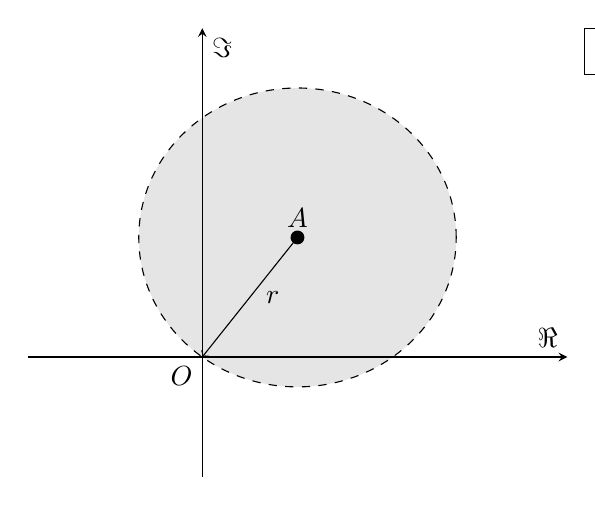
\begin{tikzpicture}[trim axis left, trim axis right]
        \pgfdeclarelayer{pre main}
        \pgfsetlayers{pre main,main}
        \begin{axis}[
            axis on top,
            domain = 0:10,
            samples = 101,
            axis y line=middle,
            axis x line=middle,
            xtick = \empty,
            ytick = \empty,
            xmax=11.5,
            xmin=-5.5,
            ymin=-4,
            ymax=11,
            xlabel = {$\Re$},
            ylabel = {$\Im$},
            legend cell align={left},
            legend pos=outer north east,
            legend style={fill=none},
            after end axis/.code={
                \path (axis cs:0,0) 
                    node [anchor=north east] {$O$};
                }
            ]

            \coordinate (O) at (0, 0);
            \coordinate[label=above:$A$] (C) at (3, 4);

            \pgfonlayer{pre main}
                \fill[black!10] (C) circle[radius=5];
            \endpgfonlayer

            \fill (C) circle[radius=2.5pt];

            \draw[<->] (O) -- (C);

            \node[anchor=west] at (1.7, 2) {$r$};

            \draw[dashed] (C) circle[radius=5];           

            \addlegendimage{line legend, black!10, line width=5pt}
            \addlegendentry{required locus};
        \end{axis}
    \end{tikzpicture}
\end{center}

\subsection{Further Use of the Argand Diagram}

Many interesting and varied problems involving complex numbers can be solved simply using an Argand diagram. For instance, one may ask what the range of $\arg z$ is, given that $z$ satisfies some other constraint, e.g. $\abs{z - \i} = 1$. Given how diverse these problems may be, there is no general approach to solving them. However, there are several tips that one should keep in mind when doing these problems:
\begin{itemize}
    \item Think geometrically! Draw out the given constraints on an Argand diagram. Most of the time, the given constraints are simply the three standard loci above (circles, perpendicular bisector and half-lines).
    \item When working with circles and an external point, drawing tangents and diameters may help. This allows one to use properties of circles (e.g. tangents are perpendicular to the radius).
    \item Keep an eye out for symmetry or similar figures.
\end{itemize}